\chapter{Oracle Aplication Express}

\section{Pengenalan Oracle APEX}

Oracle Aplication Express\cite{OracleApex} yang disebut juga HTML-DB adalah sebuah framework yang berbasis pada sebuah database dedicated (sementara ini sampai versi terbaru masih dedicated untuk Oracle DB. Oracle APEX Adalah sebuah wadah dan sarana untuk membuat aplikasi yang menggunakan database Oracle Itu sendiri, pada kelas Online pertama saya belajar banyak hal cara Menggunakan Aplikasi Oracle Apex online yang di dalam video sudah diberikan link diantaranya Request Workspace, Create Workspace, Membuat Spreadsheet Pertama.

\section{Tahapan Pembuatan Aplikasi Oracle Apex}
Langkah pertama yang harus dilakukan adalah membuka website https://apex.oracle.com, disini kita akan mendapatkan akses untuk memasuki Oracle Apllication Express, pastikan email yang dimasukkan valid untuk membuat Workspace, berikut adalah langkah langkah pembuatan Aplikasi pada Oracle APEX :

\begin{enumerate}
\item[1]Pergi ke Website Oracle APEX, https://apex.oracle.com, lalu klik Get Start For Free.

\begin{figure}[!htbp]
    \begin{center}
    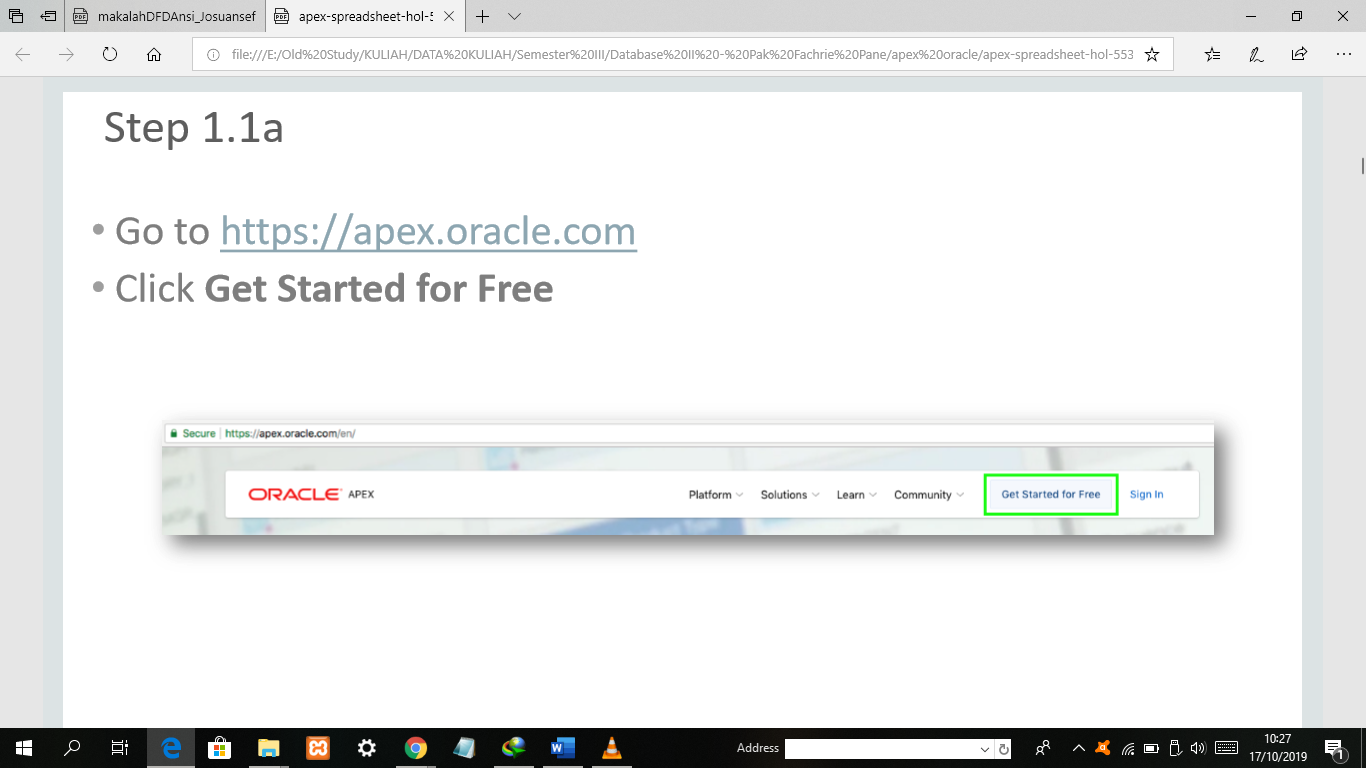
\includegraphics[scale=0.2]{figures/pict(1).png}
    \caption{\textit{Go to Website Get Start For Free.}}
    \end{center}   
    \end{figure}
    
\begin{figure}[!htbp]
\item[2]Klik Request a Free Worksace.

    \begin{center}
    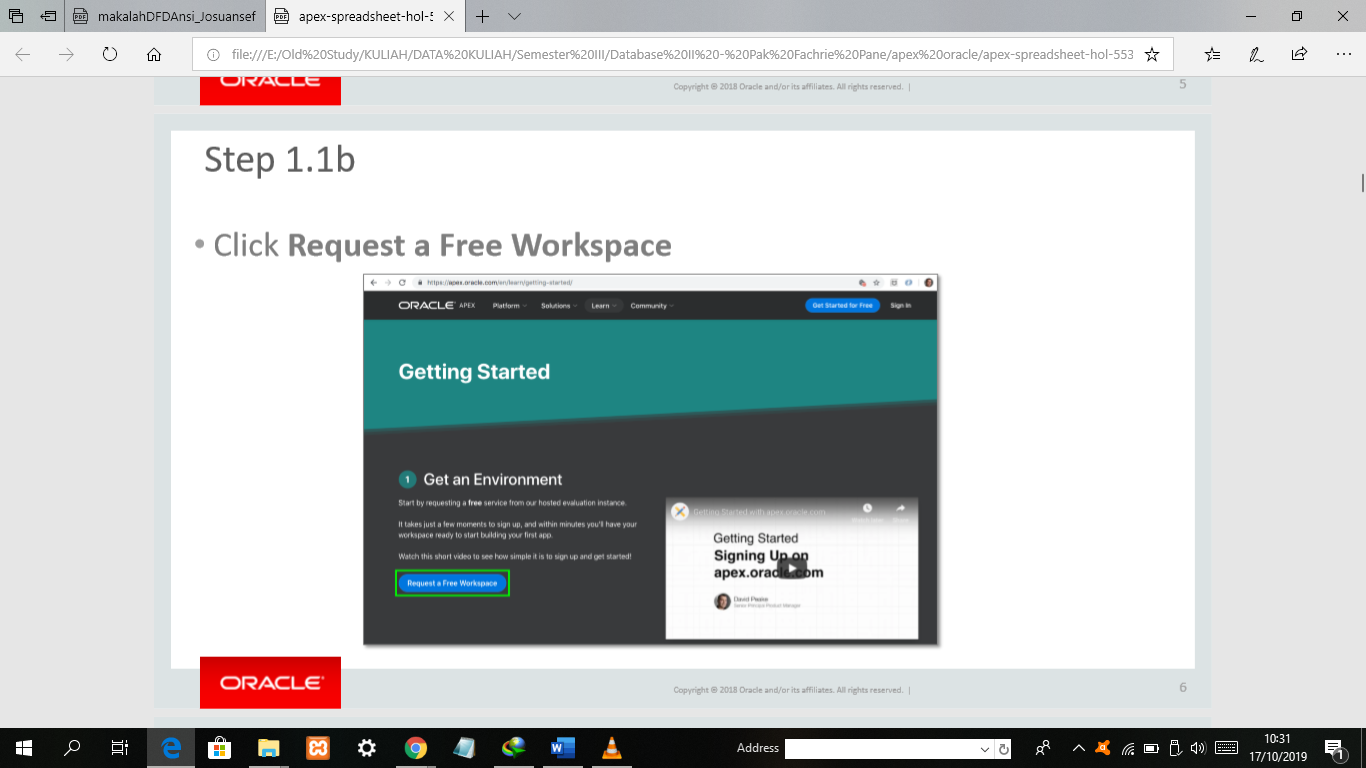
\includegraphics[scale=0.2]{figures/pict(2).png}
    \caption{\textit{Request A Free Workspace.}}
    \end{center}

\item[3]Isikan data diri anda seperti nama,email,dan workspace.

        
\item[4]Centang apakah anda pernah melakukan hal tersebut lalu next.  

      
\item[5]Isikan pada kolom tersebut bebas, mengapa anda ingin menggunakan layanan ini ?, lalu klik next.

 
\item[6] Centang Accept, lalu klik next.


\item[7] Tahapan terakhir untuk mengkonfirmasi apakah ini anda, lalu klik next.

   
\item[8] Workspace Sukses Dibuat dan Cek Email.

    \begin{center}
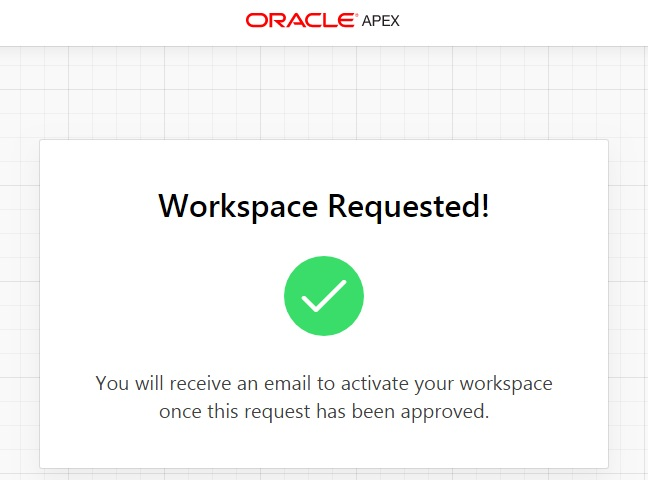
\includegraphics[scale=0.5]{figures/pict(3).jpg}
    \caption{\textit{Finish lalu Cek Email}}
        \end{center}
\label{gambar}
\end{figure}

\begin{figure}
\item[9] Workspace yang dibuat telah di Acc lalu klik continue.

    \begin{center}
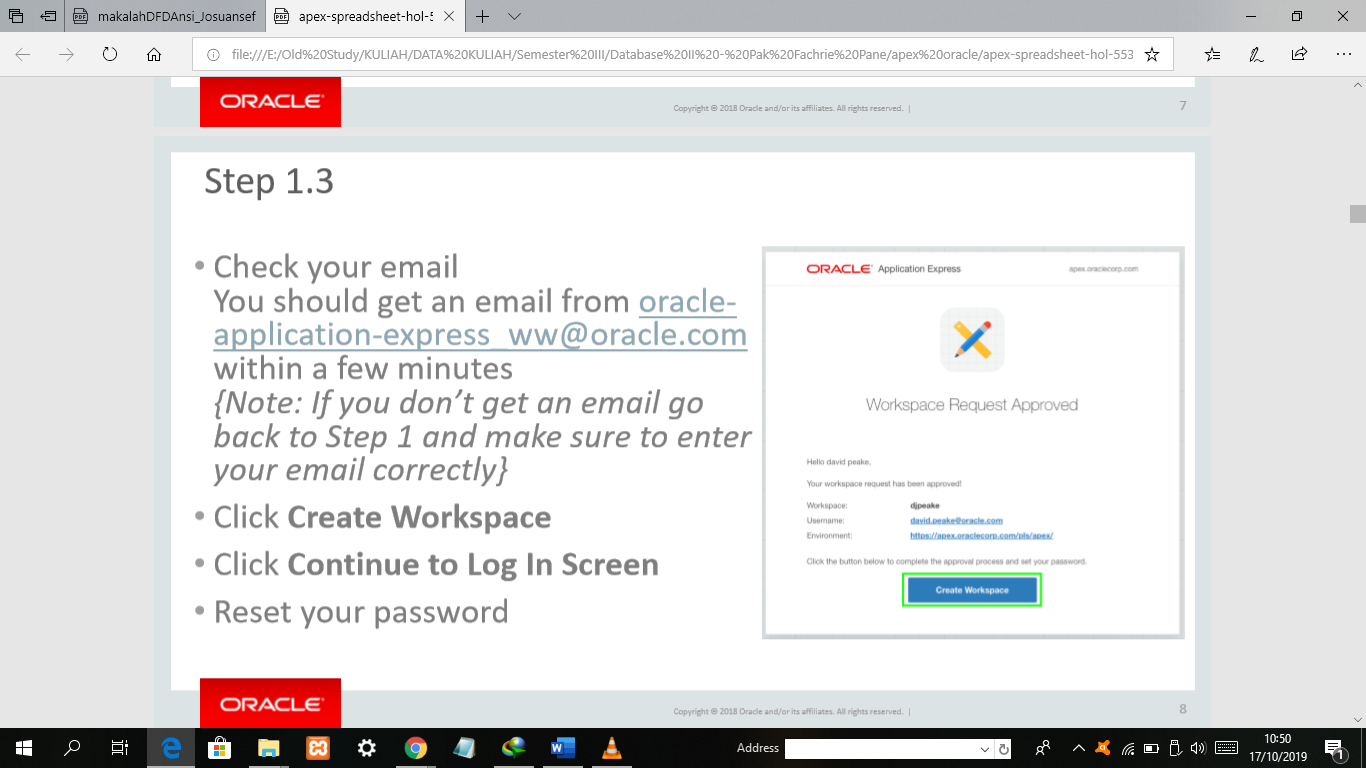
\includegraphics[scale=0.2]{figures/pict(4).png}
    \caption{\textit{Email Acc.}}
        \end{center}
\label{gambar}
\end{figure}

\begin{figure}
\item[10] Workspace baru telah dibuat setelah itu lanjutkan dengan klik sign in.

    \begin{center}
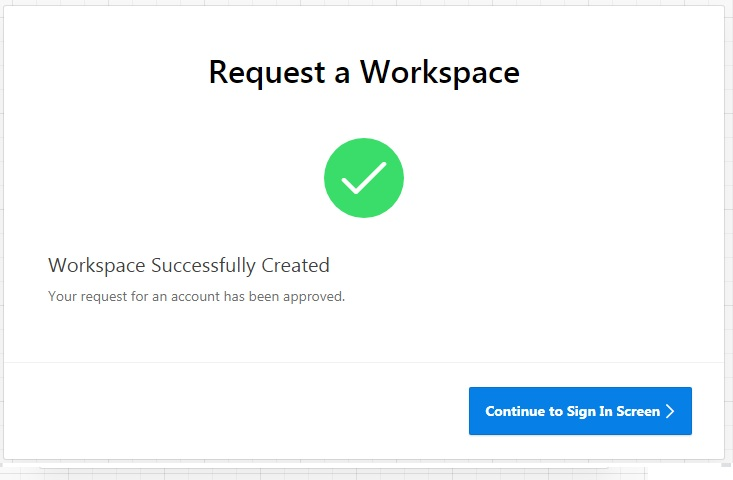
\includegraphics[scale=0.5]{figures/pict(5).jpg}
    \caption{\textit{Sukses lalu Cek Email}}
        \end{center}
\label{gambar}
\end{figure}

\begin{figure}
\item[11] Lakukan Sign in akun workspace yang baru saja di buat.

    \begin{center}
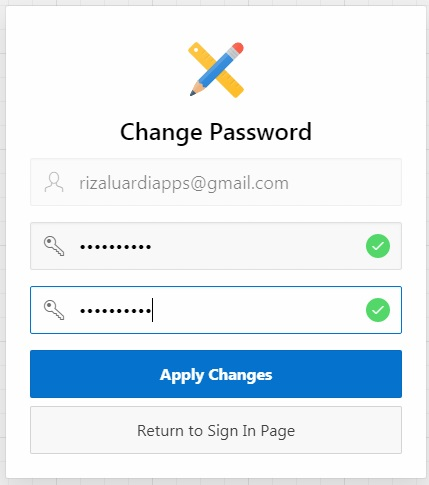
\includegraphics[scale=0.5]{figures/pict(6).jpg}
    \caption{\textit{Sign in oracle.}}
        \end{center}
\label{gambar}
\end{figure}

\begin{figure}
\item[12] sekarang kita masuk ke tampilan halaman awal aplikasi Oracle Express.

    \begin{center}
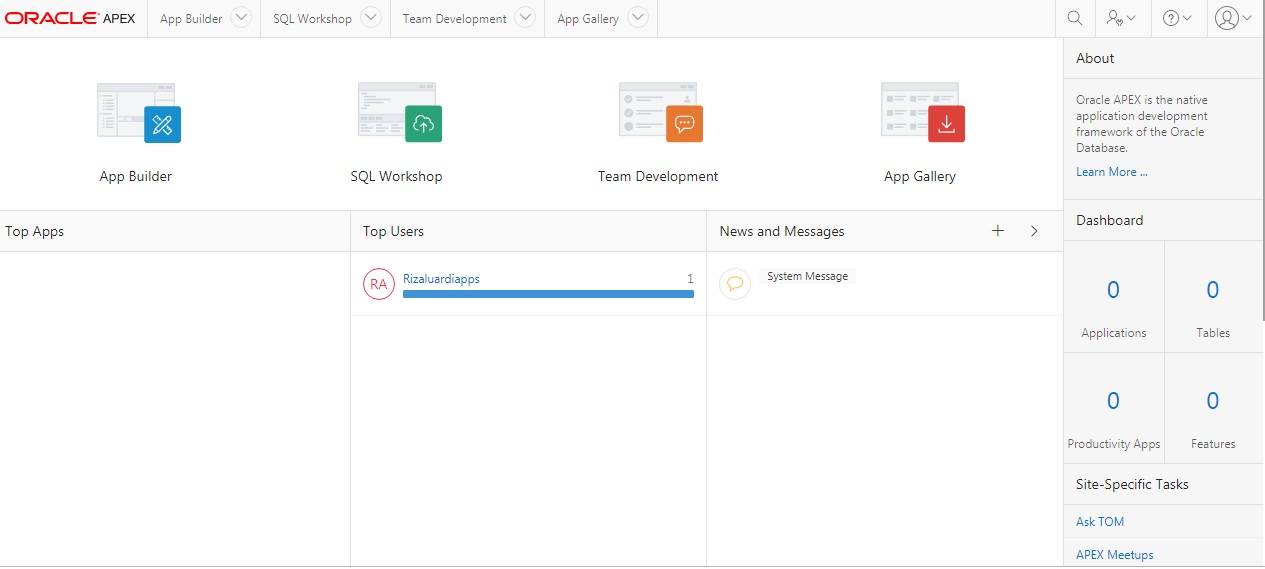
\includegraphics[scale=0.4]{figures/pict(7).jpg}
    \caption{\textit{Oracle Apex Home.}}
        \end{center}
\label{gambar}
\end{figure}

\begin{figure}
\item[13] Buka App Builder lalu klik Create New App.

    \begin{center}
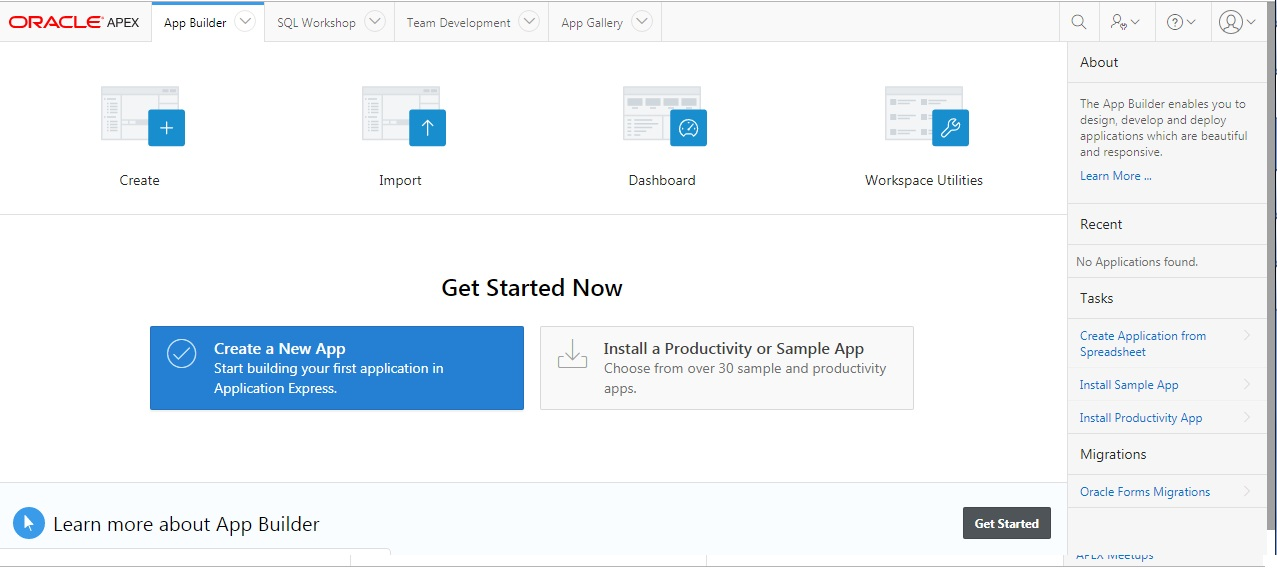
\includegraphics[scale=0.4]{figures/pict(8).jpg}
    \caption{\textit{Oracle Apex App Builder}}
        \end{center}
\label{gambar}
\end{figure}

\begin{figure}
\item[14] Klik Copy and Paste, pada select data CSV atau Sample Data Set pilih Project and Tables lalu next.

    \begin{center}
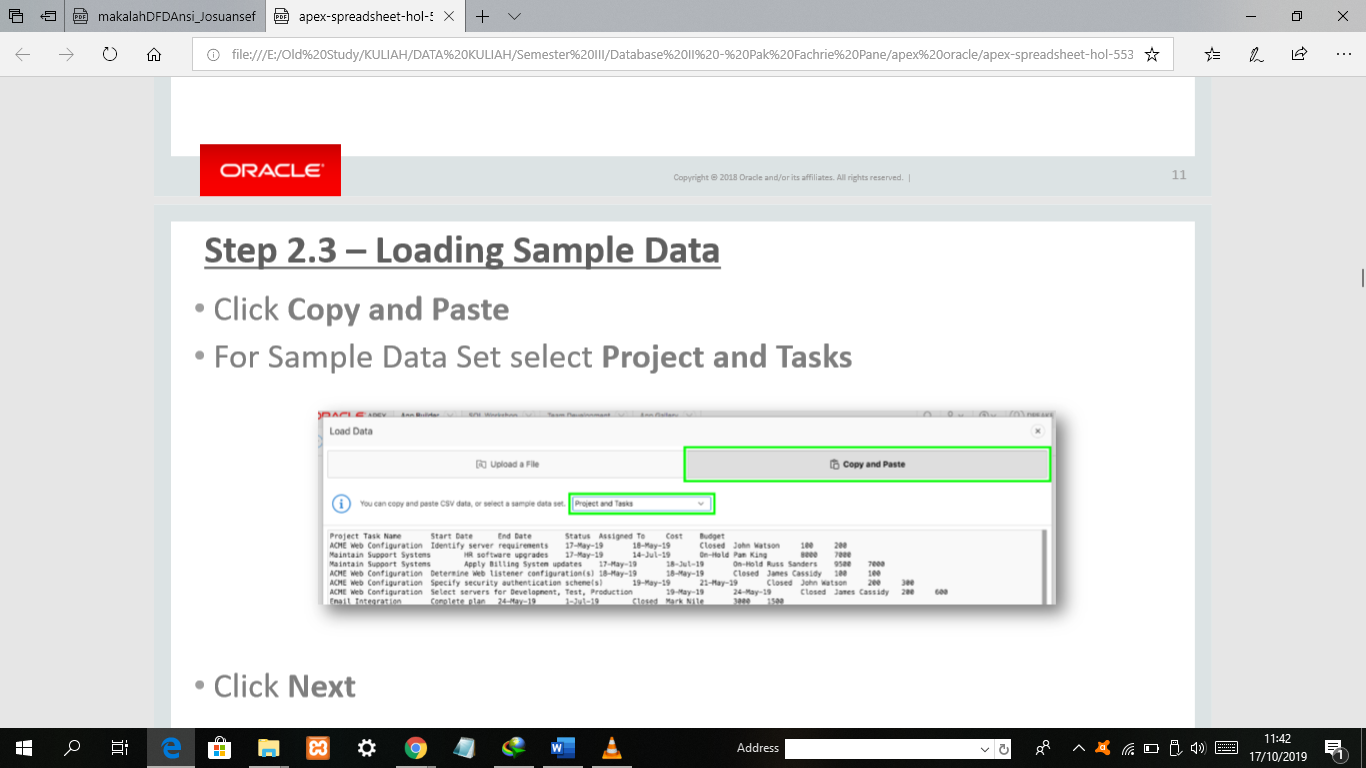
\includegraphics[scale=0.2]{figures/pict(9).png}
    \caption{\textit{Sample Data Set/ Select data CSV}}
        \end{center}
\label{gambar}
\end{figure}

\begin{figure}
\item[15] Setelah Sudah me-Load data, tampilan selanjutnya akan seperti berikut. masukkan nama tabel {SPREADSHEET}, table owner, error Table Name dan Primary Keys, lalu klik load data

    \begin{center}
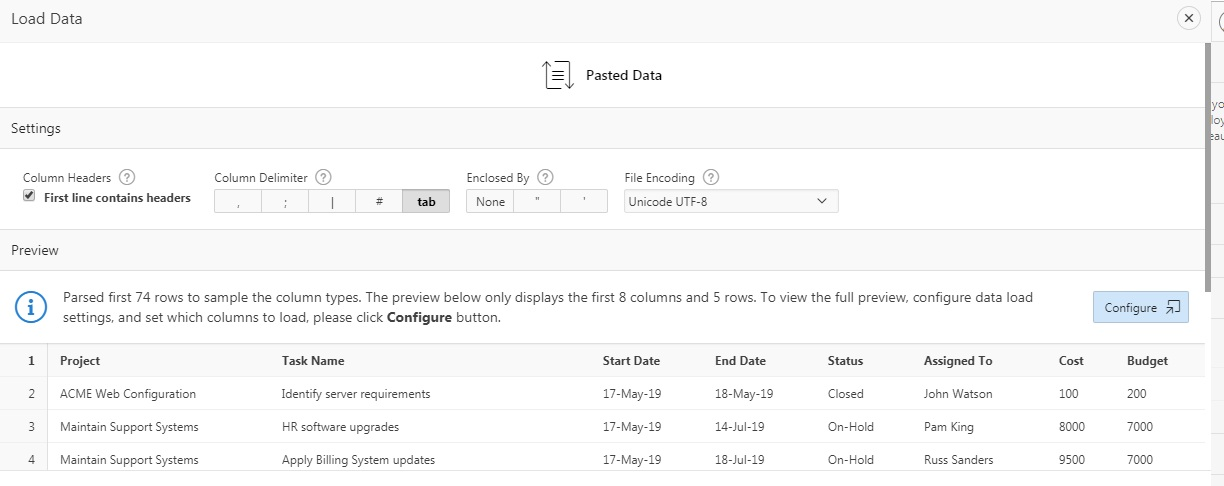
\includegraphics[scale=0.4]{figures/pict(10).jpg}
    \caption{\textit{Load Data.}}
        \end{center}
\label{gambar}
\end{figure}

\begin{figure}
    \begin{center}
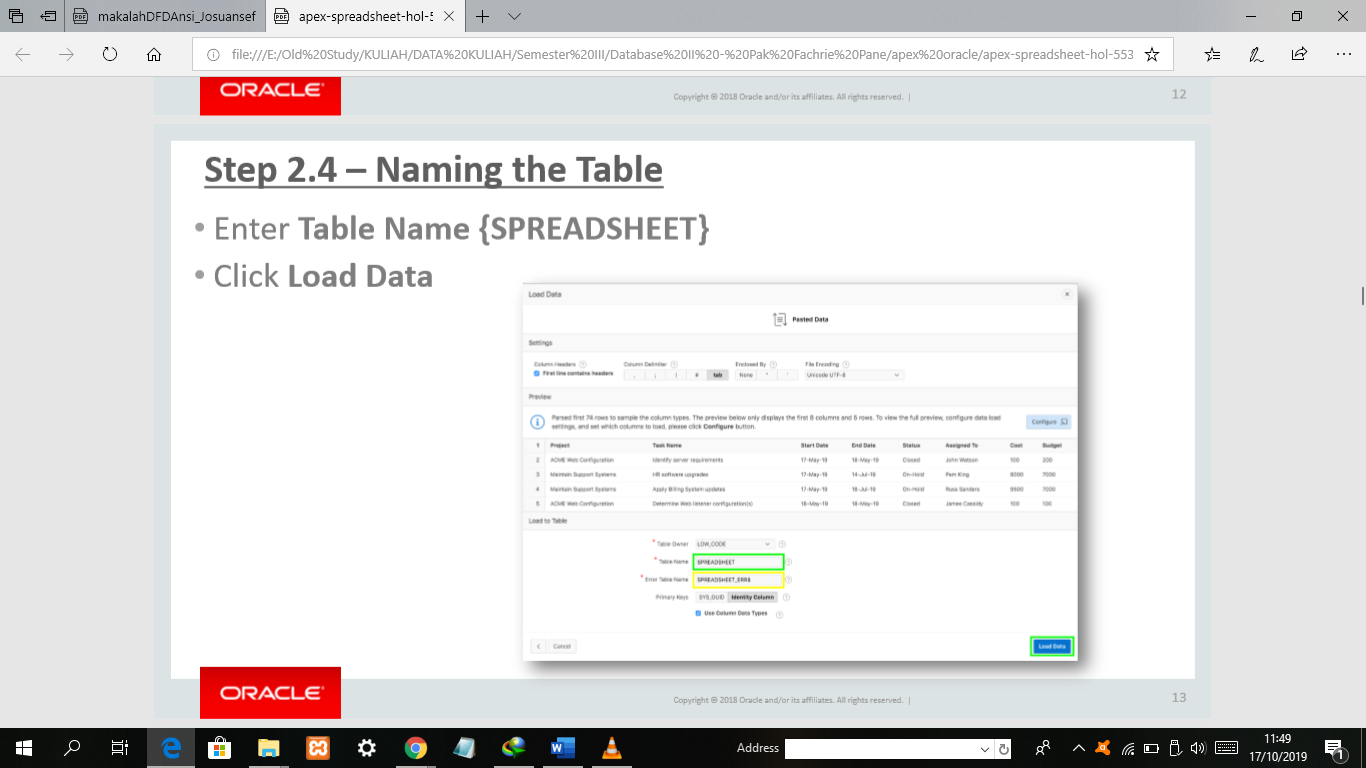
\includegraphics[scale=0.2]{figures/pict(11).png}
    \caption{\textit{Load Data 2}}
        \end{center}
\label{gambar}
\end{figure}

\begin{figure}
\item[16] Load Data Sukses , klik Continue to Create Aplication Wizard.

    \begin{center}
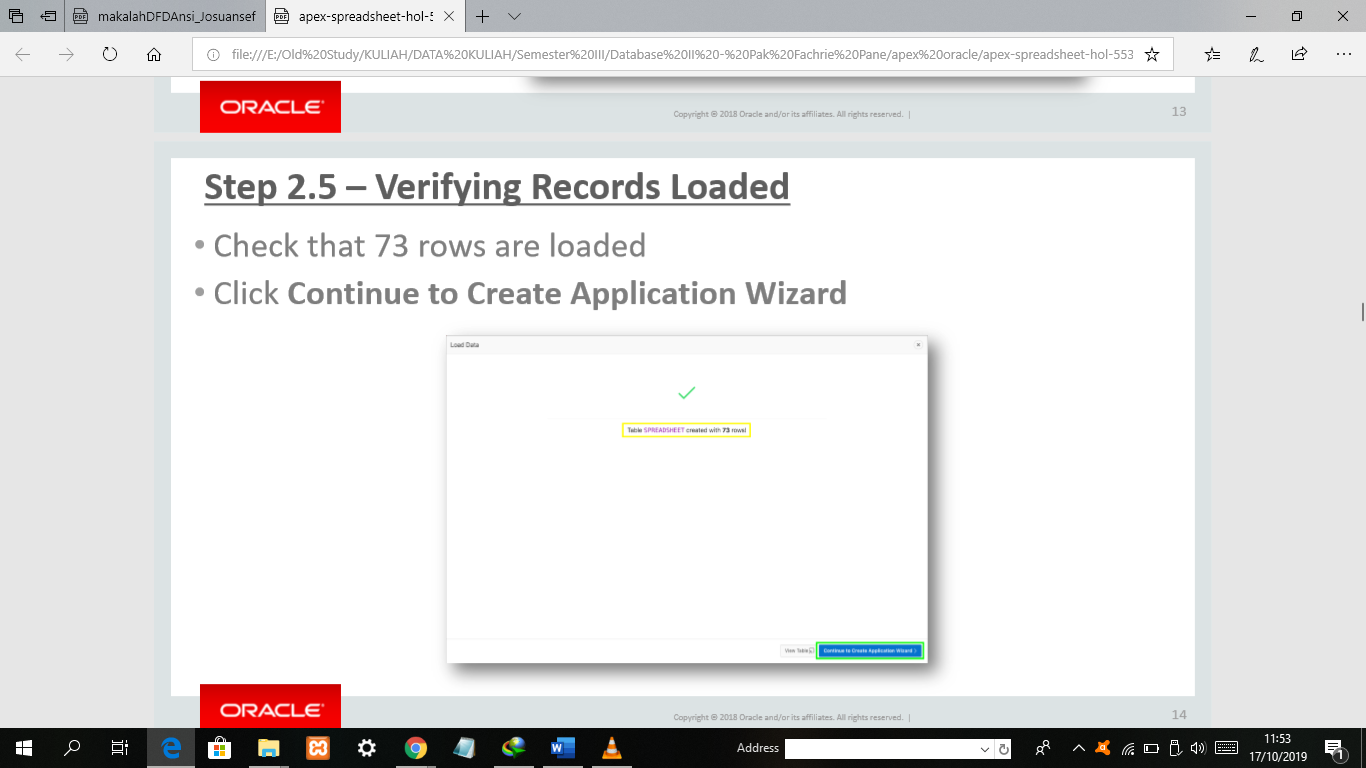
\includegraphics[scale=0.2]{figures/pict(12).png}
    \caption{\textit{Oracle Apex Load Data Success.}}
        \end{center}
\label{gambar}
\end{figure}

\begin{figure}
\item[17] Sekarang kita berada di tampilan Create an Aplication, ikuti langkah berikut, buat nama App from a Spreadsheet lalu pada Features klik Check All.

    \begin{center}
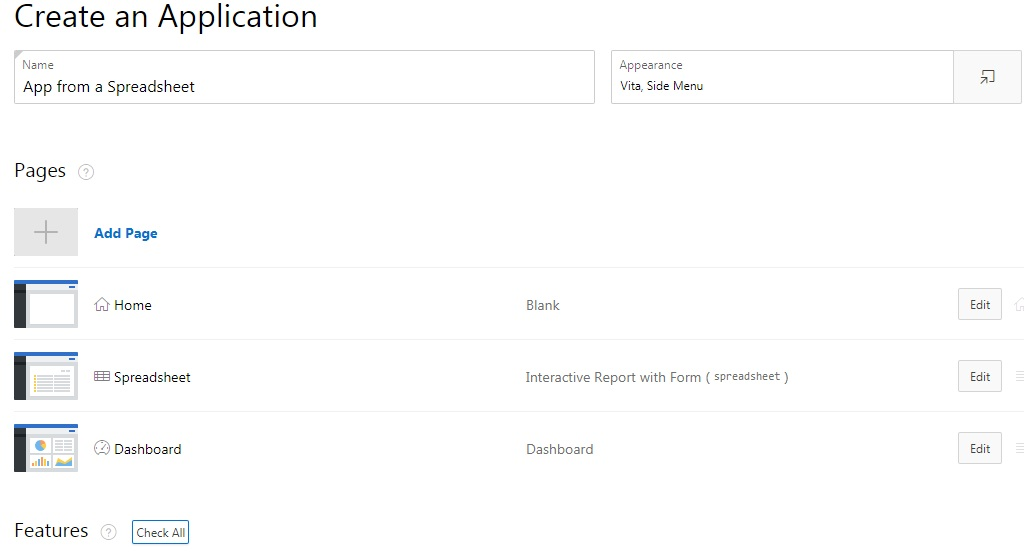
\includegraphics[scale=0.4]{figures/create1.jpg}
    \caption{\textit{Create an Aplication.}}
        \end{center}
\label{gambar}
\end{figure}


\begin{figure}
\item[18]Scroll ke bawah lalu klik Create Application .

    \begin{center}
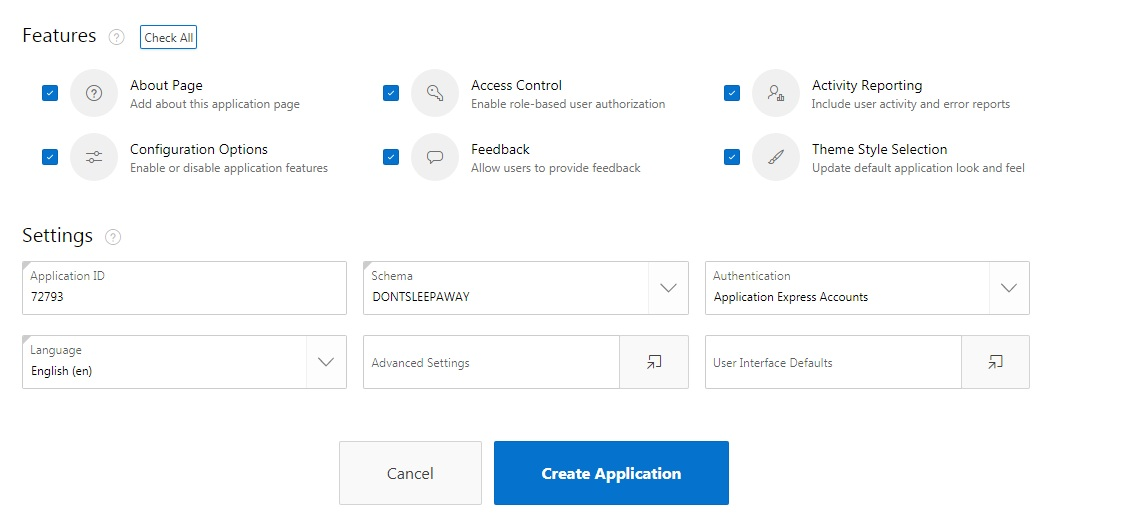
\includegraphics[scale=0.4]{figures/create2.jpg}
    \caption{\textit{Create an Application}}
        \end{center}
\label{gambar}
\end{figure}

\begin{figure}
\item[19]Tunggu beberapa saat selamat data sedang dimuat.

    \begin{center}
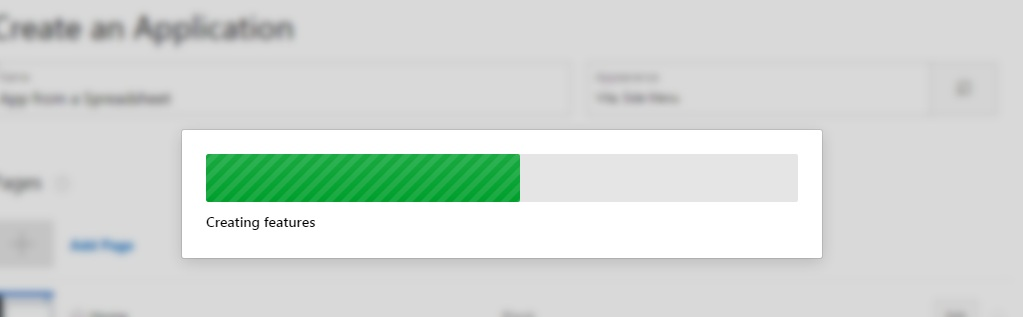
\includegraphics[scale=0.4]{figures/create3.jpg}
    \caption{\textit{Loading Data}}
        \end{center}
\label{gambar}
\end{figure}

\begin{figure}
\item[20]Sekarang kita masuk ke halaman App Builder project Spreadsheet yang telah berhasil dibuat. aplikasi yang baru dibuat akan tampil di halaman designer, setelah itu klik Run application .

    \begin{center}
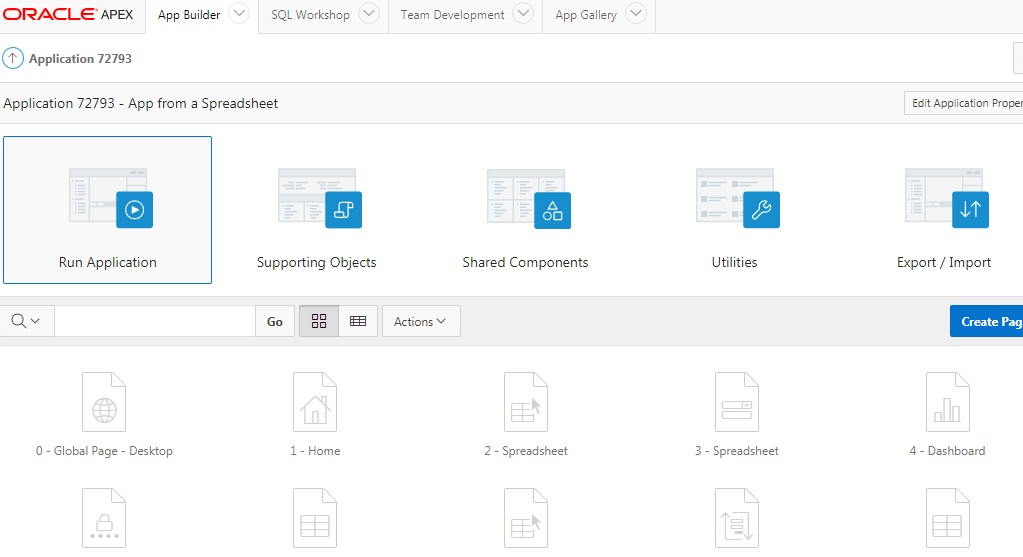
\includegraphics[scale=0.4]{figures/create4.jpg}
    \caption{\textit{App Builder Success}}
        \end{center}
\label{gambar}
\end{figure}

\begin{figure}
\item[21]Login ke Aplikasi yang baru dibuat tadi dengan menggunakan login Oracle APEX .

    \begin{center}
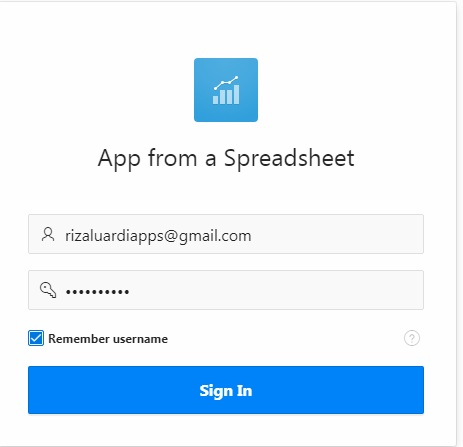
\includegraphics[scale=0.4]{figures/create5.jpg}
    \caption{\textit{Sign In Spreadsheet}}
        \end{center}
\label{gambar}
\end{figure}

\begin{figure}
\item[22]Sekarang aplikasi Oracle Apex sudah dijalankan.

    \begin{center}
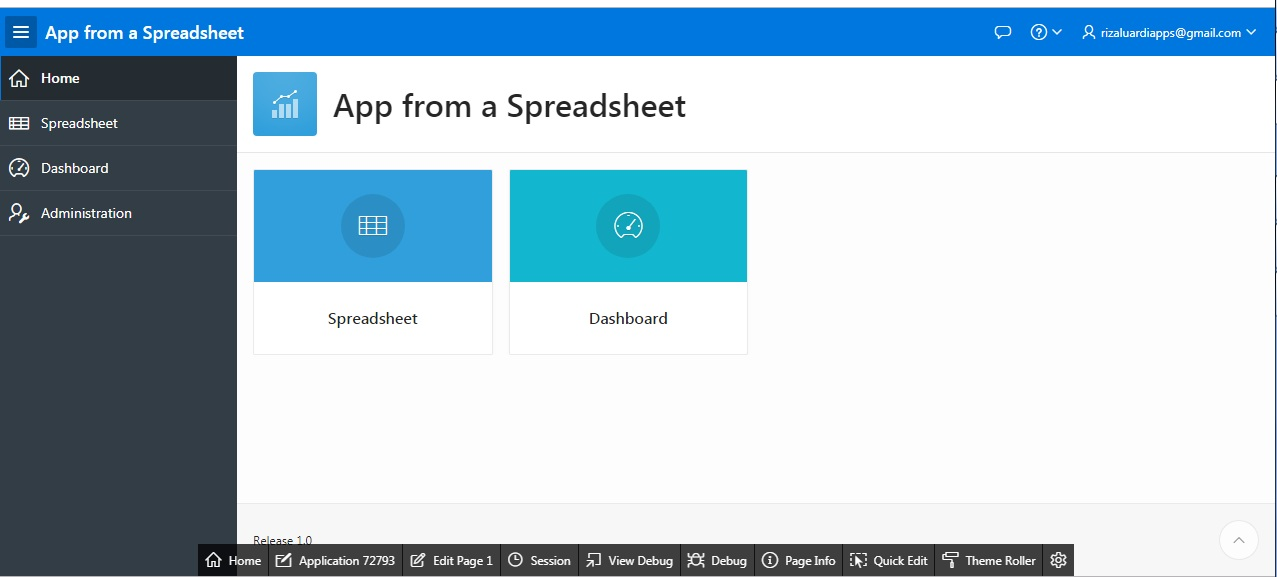
\includegraphics[scale=0.4]{figures/congratz.jpg}
    \caption{\textit{Welcome Spreadsheet}}
        \end{center}
\label{gambar}
\end{figure}

\end{enumerate}
